\chapter{\ifenglish Background Knowledge and Theory\else ทฤษฎีที่เกี่ยวข้อง\fi}

\hspace{1.27cm}การทำโครงงาน เริ่มต้นด้วยการศึกษาค้นคว้า ทฤษฎีที่เกี่ยวข้อง หรือ งานวิจัย/โครงงาน ที่เคยมีผู้นำเสนอไว้แล้ว ซึ่งเนื้อหาในบทนี้ก็จะเกี่ยวกับการอธิบายถึงสิ่งที่เกี่ยวข้องกับโครงงาน เพื่อให้ผู้อ่านเข้าใจเนื้อหาในบทถัดๆ ไปได้ง่ายขึ้น

\section{ระบบฐานข้อมูล (Database System)}
\hspace{1.27cm}ระบบฐานข้อมูล (Database System) หมายถึงโครงสร้างสารสนเทศที่ประกอบด้วย รายละเอียดของข้อมูลที่เกี่ยวข้องกันที่จะนำมาใช้ในระบบต่าง ๆ ร่วมกัน  ซึ่่งผู้ใช้สามารถจัดการกับ
ข้อมูลได้ในลักษณะต่าง ๆ ทั้งเพิ่ม ลบ หรือแก้ไขตลอดจนการเรียกดูข้อมูล ส่วนใหญ่จะเป็นการประยุกต์นำเอาระบบคอมพิวเตอร์เข้ามาช่วยในการจัดการฐานข้อมูล

ระบบฐานข้อมูล มีคำศัพท์ต่างๆที่เกี่ยวข้องดังนี้

\begin{enumerate}
  \hangindent=2em \hangafter=1
  \item เอนทิตี้ (Entity) หมายถึงสิ่งที่เราสนใจจะเก็บข้อมูล เช่น นักศึกษา อาจารย์ วิชาการ หรือห้องเรียน
  \item แอตทริบิวต์ (Attribute) หมายถึงคุณสมบัติของเอนทิตี้ เช่น ชื่อ นามสกุล หรือรหัสนักศึกษา
  \item ความสัมพันธ์ (Relationship) หมายถึงความสัมพันธ์ระหว่างเอนทิตี้ โดยที่เอนทิตี้หนึ่งสามารถมีความสัมพันธ์กับเอนทิตี้อีกเอนทิตี้หนึ่งได้ เช่น นักศึกษาสามารถลงทะเบียนเรียนในหลายวิชา และวิชาใด ๆ ก็สามารถมีนักศึกษาหลายคนลงทะเบียนเรียนได้
  \item คีย์หลัก (Primary Key) หมายถึงคีย์ที่ใช้เพื่อระบุเอนทิตี้นั้น ๆ อย่างชัดเจน และไม่สามารถซ้ำกันได้  
  \item คีย์นอก (Foreign Key) หมายถึงคีย์ที่เป็นคีย์หลักของเอนทิตี้หนึ่ง และเป็นคีย์ที่อยู่ในเอนทิตี้อีกเอนทิตี้หนึ่ง  
\end{enumerate}



\section{ไมโครเซอร์วิส (Microservices)}
\hspace{1.27cm}Microservice\cite{microservice} หรือ Microservice Architecture คือสถาปัตยกรรมการออกแบบ Service หรือก็คือออกแบบซอฟต์แวร์ โดยการที่ในชื่อมีคำว่า Micro นำหน้าอยู่ก็เพราะว่าเป็นการออกแบบที่ทำให้ Service มีขนาดเล็กเพื่อแก้ไขจุดด้อยของสถาปัตยกรรมการออกแบบอื่นๆ 

\subsection{Monolithic VS Microservice}
\hspace{1.27cm}หาก Microservice เป็นการออกแบบ Service ให้มีขนาดเล็ก การจะเทียบให้เห็นภาพชัดเจนที่สุดก็ต้องเทียบกับ Monolithic ที่เป็นระบบที่มีขนาดใหญ่ โดย Monolithic จะเป็นระบบที่มีการทำงานทั้งหมดอยู่ใน Service เดียว
% Subsection 1 text
% \clearpage
\begin{figure}[H] % 'H' forces placement exactly here
% \begin{figure}[ht] % 'ht' means place it approximately here
  \centering
  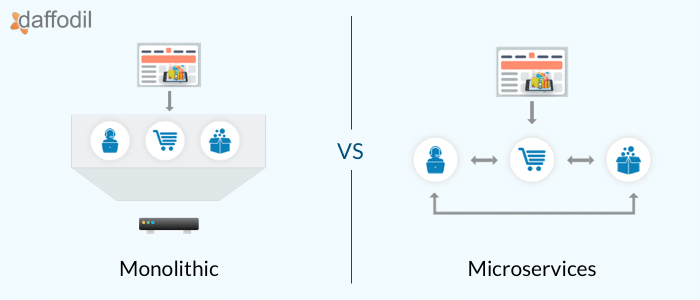
\includegraphics[width=\linewidth, keepaspectratio]{pictures/monolithic-vs-microservices.png}
  \caption[Monolithic Vs Microservice]{รูปจาก nsights.daffodilsw.com}
  % \label{fig:monolithic-vs-microservices}
\end{figure}


\subsubsection{ความแตกต่างระหว่าง Monolithic และ Microservice}
\begin{itemize}
  \item \textbf{Monolithic} เป็นชื่อของสถาปัตยกรรมการออกแบบซอฟต์แวร์หรือ Service ที่มีคนใช้งานเป็นจำนวนมากและมีมาอย่างยาวนาน โดยเป็นลักษณะของระบบที่การทำงานทุกอย่างจะรวมอยู่ในกลุ่มก้อนเดียวกัน และใช้งาน Database เดียวกัน (อย่างในภาพจะเห็นว่าเป็นเว็บไซต์ขายสินค้าที่มีฟังก์ชันจัดการผู้ใช้, ตะกร้าสินค้า และการส่งสินค้า รวมอยู่ด้วยกัน และใช้ฐานข้อมูลเดียวกัน)
  \item \textbf{Microservice}  จะออกแบบโดยแยกการทำงานที่รวมกันเป็นก้อนใหญ่ๆของแบบ Monolithic ออกมาให้เล็กลงโดยอาจจะแยกตามบริการหรือตามฟังก์ชันการทำงานเลยก็ได้ (จากในภาพฟังก์ชันทั้งสามอย่างจะแยกออกจากกัน และไม่ได้ใช้ฐานข้อมูลเดียวกันในการเก็บข้อมูลอีกต่อไป เพราะแต่ละฟังก์ชันหรือบริการที่แยกออกมามีฐานข้อมูลเป็นของตัวเอง และสามารถติดต่อกันได้ผ่าน API )
\end{itemize}




\subsubsection{ข้อดีและข้อเสียของ Microservice}
\begin{itemize}
  \item ข้อดี
  \begin{enumerate}
    \item การทำงานหลักแต่ละส่วนของระบบ ถ้าเป็นไปได้ควรแยกออกเป็น service แต่ละอัน เช่นจัดการสินค้า กับจัดการการซื้อสินค้าก็แยกกันไปเลย
    \item มีที่เก็บข้อมูลของตัวเอง
  \end{enumerate}
  \item ข้อเสีย
  \begin{enumerate}
    \item การจัดการระบบที่มีหลาย service อาจจะทำให้การจัดการระบบทำได้ยากขึ้น
    \item การทำงานของระบบที่แยกออกมาอาจจะทำให้การทำงานของระบบช้าลง
  \end{enumerate}
\end{itemize}
\clearpage

\section{Reverse Proxy}
\begin{figure}[H]
  \centering
  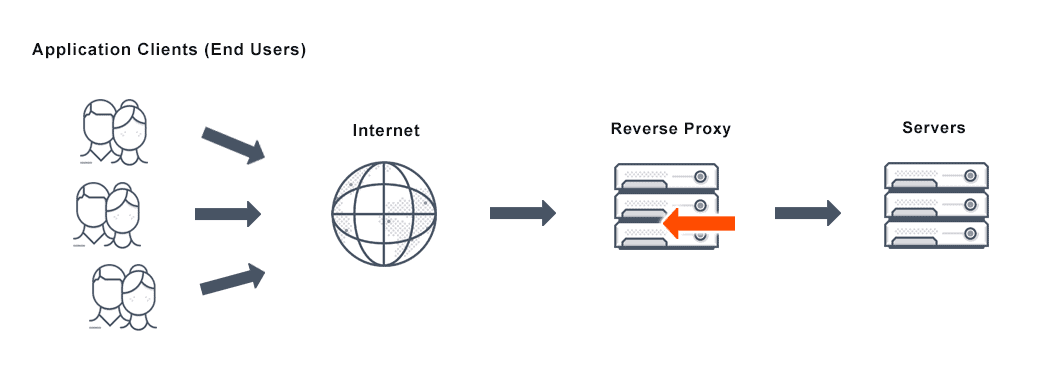
\includegraphics[width=\linewidth, keepaspectratio]{pictures/reverse_proxy.png}
  \caption[Reverse Proxy]{รูปจาก https://www.vmware.com/topics/reverse-proxy-server}
  \label{fig:reverse-proxy}
\end{figure}

\hspace{1.27cm}Reverse Proxy\cite{ReverseProxy} เป็นเซิร์ฟเวอร์พร็อกซีที่ทำหน้าที่เป็นตัวกลางระหว่าง ไคลเอนต์ (Client) และ เซิร์ฟเวอร์ต้นทาง (Origin Server) โดยไคลเอนต์จะส่งคำขอ (Request) ไปยัง Reverse Proxy และจากนั้น Reverse Proxy จะส่งคำขอนั้นไปยังเซิร์ฟเวอร์ที่เหมาะสม แล้วรับคำตอบกลับมาเพื่อส่งต่อให้ไคลเอนต์

\subsection{ประโยชน์ของการทำ Reverse Proxy}
การทำ Reverse Proxy มีประโยชน์หลายอย่างโดยประโยชน์หลักๆ จะมีดังนี้
\begin{itemize}
  \item ป้องกันการโจมตี DDoS
  \item ซ่อน IP จริงของเซิร์ฟเวอร์
  \item ใช้ SSL/TLS เพื่อเข้ารหัสข้อมูล
  \item กระจายโหลด (Load Balancing) ไปยังเซิร์ฟเวอร์หลายตัว
  \item แคชข้อมูล (Caching) ลดภาระของเซิร์ฟเวอร์ต้นทาง
\end{itemize}


\section{Hypertext Transfer Protocol (HTTP)}
\tolerance=9999
\hspace{1.27cm}HTTP \raggedright(Hypertext Transfer Protocol) เป็นโปรโตคอลสื่อสารที่ใช้ในการส่งข้อมูลระหว่างเครื่องคอมพิวเตอร์บนเครือข่ายอินเทอร์เน็ต โดย HTTP 
มีหน้าที่เป็นตัวกลา และเบราว์เซอร์ (web browsers) หรือแอปพลิเคชันอื่น ๆ 
ที่ใช้เครือข่ายอินเทอร์เน็ต งในการร้องขอและส่งข้อมูลระหว่างเว็บไซต์ (web servers)


\section{Application Programing Interface (API) }
\hspace{1.27cm}คือ การเชื่อมต่อโปรแกรมประยุกต์ ในบริบทนี้ คำว่า "Application" หมายถึงทุกซอฟต์แวร์ที่มีฟังก์ชันชัดเจน และ "Interface" ก็คือตัวประสานหรือเป็นเหมือนสัญญาที่กำหนดวิธีการซื่อสารกันระหว่าง "Application" API ทำงานใน 4 รูปแบบด้วยกัน โดยขึ้นอยู่กับเวลาและสาเหตุที่สร้าง API
\begin{enumerate}
  \item SOAP API - Simple Object Access Protocol (โปรโตคอลการเข้าถึงอ็อบเจกต์อย่างง่าย) ไคลเอ็นต์และเซิร์ฟเวอร์จะแลกเปลี่ยนข้อความโดยใช้ XML ซึ่งเป็น API ที่มีความยืดหยุ่นน้อยซึ่งเคยได้รับความนิยมมากกว่านี้ในอดีต
  \item RPC API - Remote Procedure Call (การเรียกใช้กระบวนการระยะไกล) ไคลเอ็นต์ดำเนินการฟังก์ชัน (หรือกระบวนการ) หนึ่งๆ บนเซิร์ฟเวอร์ และเซิร์ฟเวอร์ส่งผลลัพธ์กลับไปยังไคลเอ็นต์
  \item Websocket API - Web API สมัยใหม่ที่ใช้อ็อบเจกต์ JSON ในการส่งข้อมูล WebSocket API รองรับการสื่อสารสองทางระหว่างแอปไคลเอ็นต์และเซิร์ฟเวอร์ เซิร์ฟเวอร์สามารถส่งข้อความเรียกกลับไปยังไคลเอ็นต์ที่เชื่อมต่อ จึงทำให้มีประสิทธิภาพมากกว่า REST API
  \item REST API - API ที่ได้รับความนิยมและยืดหยุ่นที่สุดที่พบในเว็บไซต์ปัจจุบัน ไคลเอ็นต์ส่งคำขอไปยังเซิร์ฟเวอร์เป็นข้อมูล เซิร์ฟเวอร์ใช้ข้อมูลอินพุตจากไคลเอ็นต์นี้เพื่อเริ่มต้นฟังก์ชันภายในและส่งคืนข้อมูลเอาต์พุตกลับไปยังไคลเอ็นต์
\end{enumerate}


\section{Json Web Token (JWT)}
\hspace{1.27cm}JWT\cite{jwt}เป็นมาตรฐานแบบเปิด (RFC 7519) ที่กำหนดรูปแบบข้อมูลที่มีขนาดเล็กและสามารถตรวจสอบได้ในตัวเอง เพื่อใช้ในการส่งข้อมูลระหว่างฝ่ายต่างๆ อย่างปลอดภัยในรูปแบบของ JSON ข้อมูลนี้สามารถตรวจสอบและเชื่อถือได้ เนื่องจากมีการลงนามดิจิทัล (digitally signed)

\section{Message Queue}

\hspace{1.27cm}Message Queue\cite{messageQueue} (เรียกย่อๆว่า MQ) เป็นส่วนประกอบหนึ่งที่สำคัญในการออกแบบระบบขนาดใหญ่ โดย MQ ทำหน้าที่ในการรับ Message จากต้นทาง เก็บรักษาไว้ตามลำดับที่รับ Message เข้ามา และเปิดให้ปลายทาง มาหยิบ Message ออกไปทีละ 1 Message (หรือมากกว่า) ตามลำดับที่กำหนดไว้ตามประเภทของ Queue นั้นๆโดยที่ MQ นั้นเอง ก็มีหลากหลายประเภท หลายยี่ห้อผู้ผลิต และหลากหลายลักษณะการใช้งาน แต่ในพื้นฐานแล้ว ก็จะมีลักษณะเหมือนกัน ลองมาดูภาพการทำงานแบบคร่าวๆกันครับ


\begin{figure}[H]
  \centering
  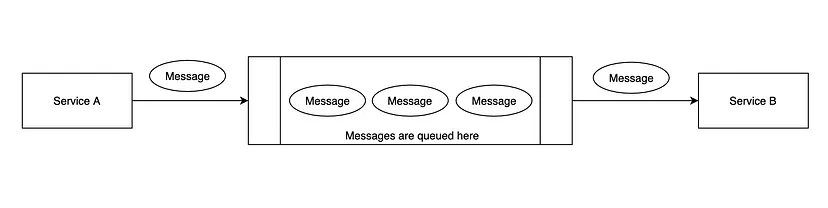
\includegraphics[width=\linewidth, keepaspectratio]{pictures/message_queue.png}
  \caption[Message Queue]\raggedright{รูปจาก https://panitw.medium.com/การใช้งาน-message-queue-pattern-65b90a6c4364}
  \label{fig:message-queue}
\end{figure}

\hspace{1.27cm}จากภาพ เราเรียก Service A ว่า Producer (ผู้ผลิต) และ Service B ว่า Consumer (ผู้บริโภค) โดย Producer จะสร้าง Message และส่งเข้าไปรอไว้ในคิว เพื่อให้ Consumer มาหยิบข้อความไปใช้ ข้อความที่ส่งเข้าไปใน MQ ก็จะถูกเก็บรักษาเอาไว้รอให้ Consumer มาหยิบโดยความเร็วข้อความที่ส่งเข้ามา อาจจะไม่เท่ากับความเร็วของข้อความที่ถูกดึงออกไป เช่นถ้า Producer ส่งข้อความทีละ 10 ข้อความต่อนาที แต่ Consumer อ่านไปทำได้ทีละ 1 ข้อความต่อนาที ก็จะทำให้มีข้อความค้างใน MQ เพิ่มขึ้นเรื่อยๆ 9 ข้อความต่อนาที
% Section 3 text. The dielectric constant\index{dielectric constant}
% at the air-metal interface determines
% the resonance shift\index{resonance shift} as absorption or capture occurs
% is shown in Equation~\eqref{eq:dielectric}:

% \begin{equation}\label{eq:dielectric}
% k_1=\frac{\omega}{c({1/\varepsilon_m + 1/\varepsilon_i})^{1/2}}=k_2=\frac{\omega
% \sin(\theta)\varepsilon_\mathit{air}^{1/2}}{c}
% \end{equation}

% \noindent
% where $\omega$ is the frequency of the plasmon, $c$ is the speed of
% light, $\varepsilon_m$ is the dielectric constant of the metal,
% $\varepsilon_i$ is the dielectric constant of neighboring insulator,
% and $\varepsilon_\mathit{air}$ is the dielectric constant of air.



% % define a command that produces some filler text, the lorem ipsum.
% % \newcommand{\loremipsum}{
% %   \textit{Lorem ipsum dolor sit amet, consectetur adipisicing elit, sed do
% %   eiusmod tempor incididunt ut labore et dolore magna aliqua. Ut enim ad
% %   minim veniam, quis nostrud exercitation ullamco laboris nisi ut
% %   aliquip ex ea commodo consequat. Duis aute irure dolor in
% %   reprehenderit in voluptate velit esse cillum dolore eu fugiat nulla
% %   pariatur. Excepteur sint occaecat cupidatat non proident, sunt in
% %   culpa qui officia deserunt mollit anim id est laborum.}\par}

% % \begin{figure}
% %   \centering

% %   \fbox{
% %      \parbox{.6\textwidth}{\loremipsum}
% %   }

% %   % To include an image in the figure, say myimage.pdf, you could use
% %   % the following code. Look up the documentation for the package
% %   % graphicx for more information.
% %   % \includegraphics[width=\textwidth]{myimage}

% %   \caption[Sample figure]{This figure is a sample containing \gls{lorem ipsum},
% %   showing you how you can include figures and glossary in your report.
% %   You can specify a shorter caption that will appear in the List of Figures.}
% %   \label{fig:sample-figure}
% % \end{figure}

% % Using \verb.\label. and \verb.\ref. commands allows us to refer to
% % figures easily. If we can refer to Figures
% % \ref{fig:walrus} and \ref{fig:sample-figure} by name in the {\LaTeX}
% % source code, then we will not need to update the code that refers to it
% % even if the placement or ordering of the figures changes.

% % \loremipsum\loremipsum

\section{Model-View-Controller (MVC)}
\hspace{1.27cm}MVC หรือ Model-View-Controller\cite{mvc} เป็นรูปแบบการออกแบบโปรแกรมที่มีการแบ่งส่วนการทำงานออกเป็น 3 ส่วน ได้แก่ Model, View และ Controller เป็น Software Design Pattern หรือแนวทางการออกแบบซอฟต์แวร์รูปแบบหนึ่งของการเขียนซอฟต์แวร์

\begin{figure}[H]
  \centering
  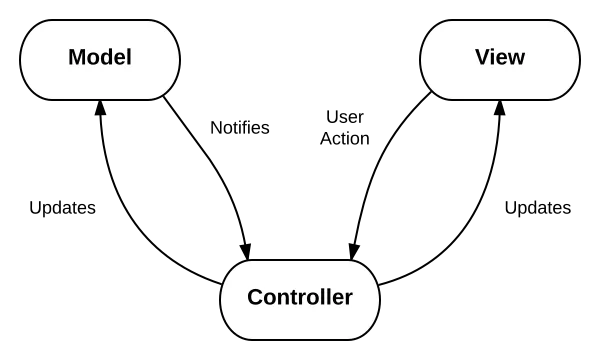
\includegraphics[width=\linewidth, keepaspectratio]{pictures/mvc.png}
  \caption[Model View Controller]{รูปจาก https://commons.wikimedia.org/wiki/File:MVC-basic.svg}
  \label{fig:mvc}
  
\end{figure}
\begin{itemize}
  \item \textbf{Model} คือส่วนที่เก็บข้อมูล และจัดการกับข้อมูล โดย Model จะไม่รู้จัก View จะส่งข้อมูลกลับไปยัง Controller เท่านั้น
  \item \textbf{View} คือส่วนที่แสดงผลข้อมูล และรับข้อมูลจากผู้ใช้ โดย View จะไม่รู้จัก Model แต่จะส่งข้อมูลกลับไปยัง Controller เท่านั้น
  \item \textbf{Controller} คือส่วนที่ควบคุมการทำงานของระบบ โดย Controller จะรับข้อมูลจาก View และส่งข้อมูลไปยัง Model และจาก Model ก็จะส่งข้อมูลกลับไปยัง View
\end{itemize}
\textbf{จุดประสงค์ของ MVC}
\begin{itemize}
  \item เพื่อแยกโค้ดออกเป็นส่วน ทำให้เราเปลี่ยนแปลงบางส่วนของโค้ดได้ โดยไม่กระทบกับส่วนอื่น ทำให้ Maintenance โค้ดทีหลังได้ง่าย
  \item ทำให้โค้ดสามารถถูกเขียนพร้อมกันโดยโปรแกรมเมอร์หลายคนได้
  \item สามารถนำโค้ดมาใช้ซ้ำได้
\end{itemize}

% % \loremipsum\loremipsum\loremipsum

% \section{Overfull hbox}

% When the \verb.semifinal. option is passed to the \verb.cpecmu. document class,
% any line that is longer than the line width, i.e., an overfull hbox, will be
% highlighted with a black solid rule:
% \begin{center}
% \begin{minipage}{10em}
% juxtaposition
% \end{minipage}
% \end{center}

% \section{\ifenglish%
% \ifcpe CPE \else ISNE \fi knowledge used, applied, or integrated in this project
% \else%
% ความรู้ตามหลักสูตรซึ่งถูกนำมาใช้หรือบูรณาการในโครงงาน
% \fi
% }

% อธิบายถึงความรู้ และแนวทางการนำความรู้ต่างๆ ที่ได้เรียนตามหลักสูตร ซึ่งถูกนำมาใช้ในโครงงาน

% \section{\ifenglish%
% Extracurricular knowledge used, applied, or integrated in this project
% \else%
% ความรู้นอกหลักสูตรซึ่งถูกนำมาใช้หรือบูรณาการในโครงงาน
% \fi
% }

% อธิบายถึงความรู้ต่างๆ ที่เรียนรู้ด้วยตนเอง และแนวทางการนำความรู้เหล่านั้นมาใช้ในโครงงาน
